%2multibyte Version: 5.50.0.2953 CodePage: 1252

\documentclass{article}
%%%%%%%%%%%%%%%%%%%%%%%%%%%%%%%%%%%%%%%%%%%%%%%%%%%%%%%%%%%%%%%%%%%%%%%%%%%%%%%%%%%%%%%%%%%%%%%%%%%%%%%%%%%%%%%%%%%%%%%%%%%%%%%%%%%%%%%%%%%%%%%%%%%%%%%%%%%%%%%%%%%%%%%%%%%%%%%%%%%%%%%%%%%%%%%%%%%%%%%%%%%%%%%%%%%%%%%%%%%%%%%%%%%%%%%%%%%%%%%%%%%%%%%%%%%%
\usepackage{amsfonts}
\usepackage{amsmath}

\setcounter{MaxMatrixCols}{10}
%TCIDATA{OutputFilter=LATEX.DLL}
%TCIDATA{Version=5.50.0.2953}
%TCIDATA{Codepage=1252}
%TCIDATA{<META NAME="SaveForMode" CONTENT="1">}
%TCIDATA{BibliographyScheme=Manual}
%TCIDATA{Created=Tuesday, September 13, 2016 11:26:35}
%TCIDATA{LastRevised=Tuesday, October 15, 2019 14:55:43}
%TCIDATA{<META NAME="GraphicsSave" CONTENT="32">}
%TCIDATA{<META NAME="DocumentShell" CONTENT="Standard LaTeX\Blank - Standard LaTeX Article">}
%TCIDATA{CSTFile=40 LaTeX article.cst}
\usepackage{enumitem}
\usepackage{floatrow}
\usepackage{graphicx} 
\usepackage{caption}

\newtheorem{theorem}{Theorem}
\newtheorem{acknowledgement}[theorem]{Acknowledgement}
\newtheorem{algorithm}[theorem]{Algorithm}
\newtheorem{axiom}[theorem]{Axiom}
\newtheorem{case}[theorem]{Case}
\newtheorem{claim}[theorem]{Claim}
\newtheorem{conclusion}[theorem]{Conclusion}
\newtheorem{condition}[theorem]{Condition}
\newtheorem{conjecture}[theorem]{Conjecture}
\newtheorem{corollary}[theorem]{Corollary}
\newtheorem{criterion}[theorem]{Criterion}
\newtheorem{definition}[theorem]{Definition}
\newtheorem{example}[theorem]{Example}
\newtheorem{exercise}[theorem]{Exercise}
\newtheorem{lemma}[theorem]{Lemma}
\newtheorem{notation}[theorem]{Notation}
\newtheorem{problem}[theorem]{Problem}
\newtheorem{proposition}[theorem]{Proposition}
\newtheorem{remark}[theorem]{Remark}
\newtheorem{solution}[theorem]{Solution}
\newtheorem{summary}[theorem]{Summary}
\newenvironment{proof}[1][Proof]{\noindent\textbf{#1.} }{\ \rule{0.5em}{0.5em}}
%\input{tcilatex}
\begin{document}


\begin{center} 
{\Large Problem Set 6}
\end{center}


\begin{exercise}%EX 9.1 SW
Suppose that you have just read a careful statistical study of the effect of improved health of children on their test scores at school. Using data from a project in a West African district in 2000, the study concluded that students who received multivitamin supplements performed substantially better at school. Use the concept of external validity to determine if these results are likely to apply to India in 2000, the United Kingdom in 2000, and West Africa in 2015.
\end{exercise}
\vspace{.5cm}

\begin{exercise} %EX 9.3 SW
Labor economists studying the determinants of women’s earnings discovered a puzzling empirical result. Using randomly selected employed women, they regressed earnings on the women’s number of children and a set of control variables (age, education, occupation, and so forth). They found that women with more children had higher wages, controlling for these other factors. Explain how sample selection might be the cause of this result.
\end{exercise}
\vspace{.5cm}



\begin{exercise}%EX9.5 SW
The demand for a commodity is given by $Q = \beta_0 + \beta_1P + u$, where $Q$ denotes quantity, $P$ denotes price, and $u$ denotes factors other than price that determine demand. Supply for the commodity is given by $Q = \gamma_0 + \gamma_1P + v$, where $v$ denotes factors other than price that determine supply. Suppose $u$ and $v$ both have a mean of $0$, have variances $\sigma_u^2$ and $\sigma_v^2$, and are mutually uncorrelated.
    \begin{enumerate}[label=\alph*)]
        \item Solve the two simultaneous equations to show how $Q$ and $P$ depend on $u$ and $v$.
        \item Derive the means of $P$ and $Q$.
        \item Derive the variance of $P$, the variance of $Q$, and the covariance between $Q$ and $P$.
        \item A random sample of observations of $(Q_i, P_i)$ is collected, and $Q_i$ is regressed on $P_i$. (That is, $Q_i$ is the regressand, and $P_i$ is the regressor.) Suppose the sample is very large.
        \begin{enumerate}[label=\roman* --]
            \item Use your answers to (b) and (c) to derive values of the regression coefficients.    
            \item A researcher uses the slope of this regression as an estimate of the slope of the demand function ($\beta_1$). Is the estimated slope too large or too small?
        \end{enumerate}
    \end{enumerate}
\end{exercise}
\vspace{.5cm}


\begin{exercise}%EX9.13 SW
Assume that the regression model $Y_i = \beta_0 + \beta_1X_i + u_i$ satisfies the least squares assumptions. You and a friend collect a random sample of 300 observations on $Y$ and $X$.
\begin{enumerate}[label=\alph*)]
    \item Your friend reports that he inadvertently scrambled the $X$ observations for 20\% of the sample. For these scrambled observations, the value of $X$ does not correspond to $X_i$ for the $i$th observation; rather, it corresponds to the value of $X$ for some other observation. The measured value of the regressor, $\tilde{X}_i$, is equal to $X_i$ for 80\% of the observations, but it is equal to a randomly selected $X_j$ for the remaining 20\% of the observations. You regress $Y_i$ on $\tilde{X}_i$. Show that $\mathbb{E}(\hat{\beta}_1)=.8\beta_1$.
    \item Explain how you could construct an unbiased estimate of $\beta_1$ using the OLS estimator in (a).
    \item Suppose now your friend tells you that the X’s were scrambled for the first 60 observations but that the remaining 240 observations are correct. You estimate $\beta_1$ by regressing $Y$ on $X$, using only the correctly measured 240 observations. Is this estimator of $\beta_1$ better than the estimator you proposed in (b)? Explain
\end{enumerate}
\end{exercise}
\vspace{.5cm}

\begin{exercise}%EX9.10 SW
Read the following text, and discuss the internal and external validity as a causal effect of the relationship between age and healthcare expenditures, considering both models 1 and 3.\\[1em]

``In Western Europe, the number of old people in the total population is increasing on average, with a greater proportion of the post-World War II “baby boom” generation reaching retirement age. This has led to researchers becoming increasingly interested in the impact of ageing on healthcare expenditures (HCE), which refers to the amount spent on improving people’s health and on health-related issues, in recent decades. Initial estimates published by the Organisation for Economic Co-operation and Development (OECD) painted a very pessimistic picture: because older people had, on average, higher HCE, an ageing population would place an associated upward pressure on public finances.

Intuitively, this seems to make sense. However, other researchers noticed a problem with this logic. If people age more healthily, what does this mean for HCE? A consensus emerged in the academic literature that what determines HCE is not ageing per se, but an individual’s proximity to death (“time-to-death”, or TTD). In terms of these expenditures, an 80 year old who dies at age 85 is more similar to a 70 year old who dies at age 75, than to another 80 year old who dies at the age of 100. Under this logic, ageing itself became termed a “red herring” in explaining HCE—that is, something that acts as a proxy for their actual determinants.

Time-to-death is regarded as omitted variable in previous regressions explaining HCE. When carrying out regressions of healthcare expenditures, the dependent variable employed is generally the logarithm of HCE, or a “log-transform” of HCE. An example of such a regression is evident in a 2015 study that was conducted on two samples of around 40,000 individuals each, from England, a) who used inpatient health care during 2005–06 and died by 2011–12 and b) who had some hospital utilization since 2005–06 but died in 2011–12. Based on the data from this study, the following table presents the results of a regression with a dependent variable of HCE for men in England between 2005–06 and 2011–12 (Howdon and Rice, 2018).

How do we interpret this output? It is important to remember that our dependent variable is not HCE, but their log transform, and that we are dealing with age and age1 as parameters. So using the coefficients from column (1), we compute the average percentage increase in healthcare expenditures for ageing from 80 to 81 as, $1 \times -0.1459 + (81^2 - 80^2) \times 0.00010 = 0.00151$, or a 0.151\% increase.

What happens when we include (the log of) TTD? We observe in column (2) that the age and age coefficients fall in absolute terms, there is a reduction in statistical significance attached to these coefficients, and that log(TTD) is highly significant in explaining log(HCE). This suggests that TTD is indeed an omitted variable in this regression. Since both of these variables are log-transformed, our results suggest that being 1\% further away from death (a 1\% increase in TTD) is associated with an average decrease in HCE of around 0.42\%. But is this the end of the story?

Further research has pointed to TTD itself as a “red herring,” with TTD itself merely proxying for individual morbidity. Measures of morbidity, under this logic, would be an omitted variable in such regressions—and this would be important in predicting future HCE if people not only age more healthily, but approach death more healthily! And this is exactly what we observe in column (3): the inclusion of morbidity controls reduces both the size and statistical significance of TTD and age-related coefficients, suggesting that TTD indeed proxies for morbidity. It is important to remember that determining the relevant variables to include in regression analysis depends on the exact nature of the question you are trying to answer.''

\begin{figure}[tbp]
\caption*{}
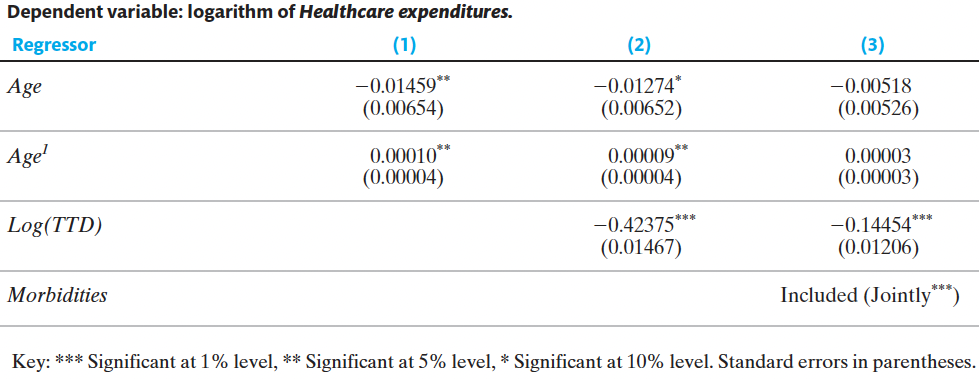
\includegraphics[width=\linewidth]{images/ps5ex5.png}
\end{figure}
\end{exercise}


\begin{exercise}%EX9.12 SW
    Consider the one-variable regression model $Y_i = \beta_0 + \beta_1 X_i + u_i$, and suppose it satisfies the least squares assumptions. The regressor $X_i$ is missing, but data on a related variable, $Z_i$, are available, and the value of $X_i$ is estimated using $\tilde{X}_i = \mathbb{E}(X_i\mid Z_i)$. Let $w_i = \tilde{X}_i - X_i$.
    \begin{enumerate}[label=\alph*)]
    \item Show that $\tilde{X}_i$ is the minimum mean square error estimator of $X_i$ using $Z_i$. That is, let $\hat{X}_i=g(Z_i)$ be some other guess of $X_i$ based on $Z_i$ and show that $\mathbb{E}[(\hat{X}_i-X_i)^2]\geq\mathbb{E}[(\tilde{X}_i-X_i)^2]$.
    \item Show that $\mathbb{E}(w_i \mid \tilde{X}_i)=0$
    \item Suppose that $\mathbb{E}(u_i \mid Z_i)=0$ and that $\tilde{X}_i$ is used as the regressor in place of $X_i$. Show that $\hat{\beta}_1$ is consistent. Is $\hat{\beta}_0$ consistent too?
    \end{enumerate}
\end{exercise}

\end{document}
